\documentclass[12pt]{article}
    \usepackage[margin=1in]{geometry}
    \usepackage{mdframed}
    \usepackage{subcaption}
    \usepackage{caption}
    \usepackage{amssymb}
    \usepackage{amsmath}
    \usepackage{mathtools}

    % Custom colors
    \usepackage{color}
    \definecolor{deepblue}{rgb}{0,0,0.5}
    \definecolor{deepred}{rgb}{0.6,0,0}
    \definecolor{deepgreen}{rgb}{0,0.5,0}
    % Default fixed font does not support bold face
    \DeclareFixedFont{\ttb}{T1}{txtt}{bx}{n}{12} % for bold
    \DeclareFixedFont{\ttm}{T1}{txtt}{m}{n}{12}  % for normal
    \usepackage{listings}
    \usepackage{url}

    \usepackage{hyperref}

    \usepackage{booktabs}
    
    \usepackage{tikz}
    \usetikzlibrary{shapes,arrows,automata,positioning,cd}
    \tikzset{
      cfgedge/.style   = {black, ->, >=stealth},
      forward/.style = { blue, ->, >=angle 45},
      backward/.style = { red, densely dashed, ->, >=latex' },
      backwardleft/.style = { red, densely dashed, <-, >=latex' },
      hasse/.style   = {black },
    }
    \usepackage{xcolor}
    
    \newcommand{\cfgarrow}{\mathbin{\tikz[baseline]\draw[cfgedge,yshift=0.6ex] (0,0) -- (.9em,0);}}
    \newcommand{\forwardarrow}{\mathbin{\tikz[baseline]\draw[forward,yshift=0.6ex] (0,0) -- (1em,0);}}
    \newcommand{\backwardarrow}{\mathbin{\tikz[baseline]\draw[backward,yshift=0.6ex] (0,0) -- (.95em,0);}}
  \newcommand{\dom}{\underline{\gg}}
    
    
    \begin{document}
    \lstset{
    language=C,
    basicstyle=\ttfamily\small,
    keywordstyle=\ttb\color{deepblue}\small,
    emph={foo,bar,assert,baz},          % Custom highlighting
    emphstyle=\ttb\color{deepred}\small,    % Custom highlighting style
    stringstyle=\color{deepgreen}\small,
    frame=tb,                         % Any extra options here
    numbers=left,
    stepnumber=1,
    showstringspaces=false            % 
    }
    
    \begin{center}
        \bigskip
        {\LARGE ECS 240 Programming Languages} \medskip
                
        {\Large Homework 5} \bigskip
    
    \end{center}
    
    \section*{About This Assignment}
    
    \begin{itemize}
        \item This assignment tests you on your understanding of abstract interpretation.
        \item To complete the assignment 
        (i)~modify \texttt{hw5.tex}, 
        (ii)~create the corresponding PDF document (using pdflatex, for example), and 
        (iii)~submit the pdf electronically via Gradescope by the due date; 
        see \href{https://www.gradescope.com/get_started#student-submission}{this page} and
        \href{http://gradescope-static-assets.s3-us-west-2.amazonaws.com/help/submitting_hw_guide.pdf}{this document}.
        Your assignment will not be graded and you will receive
        no points if you do not follow these instructions. 
  \item \textbf{When submitting the assignment on Gradescope, please mark which page
    corresponds to each question on the assignment.} Your assignment will not be graded and you will receive
    no points if you do not follow these instructions. 
  \item The \LaTeX\ source has \texttt{TODO}~comments to clearly
    indicate where changes need to be made. 
  \item The \verb=\vspace= commands can be safely commented out.
  \item This assignment can be worked on in a group of at most three. Enter
  the names and email addresses of the team members in the space provided
  below.
\end{itemize}

\begin{mdframed}
  Team members:
  \begin{itemize}
    %TODO
    \item Soham Kolhatkar, sakolhatkar@ucdavis.edu % Enter name and email address of first team member.
    \item Divyansh Rajesh Jain, drajeshjain@ucdavis.edu % Comment out this line if working individually.
    
  \end{itemize}
\end{mdframed}
  
  \newpage
  \begin{enumerate}



\item  (5 points) Consider the following partial order represented by its Hasse diagram:
\begin{center}
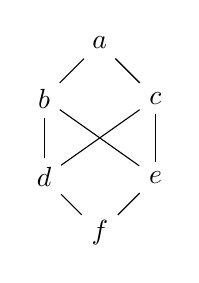
\begin{tikzpicture}[auto, node distance=1cm
    ] 
    \node (a) {$a$};
    \node [below left of=a] (b) {$b$};
    \node [below right of=a] (c) {$c$};
    \node [below of=b] (d) {$d$};
    \node [below of=c] (e) {$e$};
    \node [below right of=d] (f) {$f$};
   
    
    \path (a) edge[hasse] (b); 
    \path (a) edge[hasse] (c); 
    \path (b) edge[hasse] (d); 
    \path (d) edge[hasse] (f);
    \path (a) edge[hasse] (c);
    \path (c) edge[hasse] (e);
    \path (e) edge[hasse] (f);
    \path (b) edge[hasse] (e);
    \path (c) edge[hasse] (d);      
\end{tikzpicture}
\end{center}
 State whether \textbf{True} or \textbf{False},
 and \textbf{justify your answer}:
 \emph{The above partial order is a complete lattice.}
 \begin{mdframed}
    %\vspace{2em}
    %% TODO Comment out the correct answer.
    %\textbf{True} 
    \textbf{False}

    The above partial order is \textbf{not} a complete lattice because of the cross edge from $d$ to $c$ and the cross edge from $e$ to $b$. We know for a complete lattice to exist, all subsets in the partial order must have both greatest lower bounds and least upper bounds. We also know that the least upper bound is an element such that for upper bounds $u$, the LUB $\leq$ $u$.
    
    However when trying to find the least upper bound between $d,e$, we can see that both $b$ and $c$ are the smallest upper bounds for the subset $d,e$. If we call all upper bounds $U$, this means  $b \leq U$. This also means $c \leq U$. This implies that $b \leq c$ and $c \leq b$. However, this can only be possible if $c == b$, which we know is not true. This violates the antisymmetry property, therefore $d,e$ do not have a least upper bound, which violates the condition of a complete lattice that all subsets must have a LUB and GLB, so it is not a complete lattice. 
    
\end{mdframed}
\newpage

\item  (20 points) 
Let $(C, \gamma, \alpha, A)$ be a Galois connections between complete lattices 
$(C, \leq)$ and $(A, \sqsubseteq)$.

For each of the following state whether \textbf{True} or \textbf{False}; 
if True provide a proof, and if false, provide a counterexample in the form 
of a Galois connection explaining why it does not satisfy the given proposition: 



\begin{enumerate}
  \item 
 \emph{$\alpha ( c_1 \sqcup c_2 ) = \alpha(c_1) \sqcup \alpha(c_2)$, for all $c_1, c_2 \in C$}
 \begin{mdframed}

    %% TODO Comment out the correct answer.
    %%\textbf{True}

    \textbf{False}

    Left is concrete lattice, right is abstract lattice

    \begin{tikzpicture}[>=Stealth, thick, node distance=1.5cm]

        % Concrete lattice (left)
        \node (topC) at (0,4.5) {$\top$};
        \node (c3) at (0,3) {$c_3$};
        \node (c2) at (-1,1.5) {$c_2$};
        \node (c1) at (1,1.5) {$c_1$};
        \node (botC) at (0,0) {$\bot$};
        
        \draw (topC) -- (c3);
        \draw (c3) -- (c2);
        \draw (c3) -- (c1);
        \draw (c2) -- (botC);
        \draw (c1) -- (botC);
        
        % Abstract lattice (right)
        \node (topA) at (5,4.5) {$\top$};
        \node (a4) at (5,3.5) {$a_4$};
        \node (a3) at (5,2.5) {$a_3$};
        \node (a2) at (4.2,1.5) {$a_2$};
        \node (a1) at (5.8,1.5) {$a_1$};
        \node (botA) at (5,0) {$\bot$};
        
        \draw (topA) -- (a4) -- (a3);
        \draw (a3) -- (a2);
        \draw (a3) -- (a1);
        \draw (a2) -- (botA);
        \draw (a1) -- (botA);
        

        
    \end{tikzpicture}

    \begin{center}
    \begin{minipage}{0.45\textwidth}
    \centering
    \textbf{Abstraction function \( \alpha \)}\\[0.5em]
    \begin{tabular}{|c|c|}
    \hline
    \( c \in C \) & \( \alpha(c) \in A \) \\
    \hline
    \( \bot \) & \( \bot \) \\
    \( c_1 \) & \( a_1 \) \\
    \( c_2 \) & \( a_2 \) \\
    \( c_3 \) & \( a_4 \) \\
    \( \top \) & \( \top \) \\
    \hline
    \end{tabular}
    \end{minipage}
    \hspace{1cm}
    \begin{minipage}{0.45\textwidth}
    \centering
    \textbf{Concretization function \( \gamma \)}\\[0.5em]
    \begin{tabular}{|c|c|}
    \hline
    \( a \in A \) & \( \gamma(a) \in C \) \\
    \hline
    \( \bot \) & \( \bot \) \\
    \( a_1 \) & \( \ c_1 \) \\
    \( a_2 \) & \( \ c_2 \) \\
    \( a_3 \) & \( \ c_3 \) \\
    \( a_4 \) & \( \top \) \\
    \( \top \) & \( \top \) \\
    \hline
    \end{tabular}
    \end{minipage}
    \end{center}

    
\end{mdframed}


\item 
 \emph{$\alpha ( c_1 \sqcap c_2 ) = \alpha(c_1) \sqcap \alpha(c_2)$, for all $c_1, c_2 \in C$}
 \begin{mdframed}
    
    %% TODO Comment out the correct answer.
    %\textbf{True} 
     \textbf{False}

\begin{tikzpicture}[>=Stealth, thick, node distance=1.5cm]

    % Abstract lattice (left) - flipped vertically
    \node (topC) at (0,-4.5) {$\bot$};
    \node (c3) at (0,-3) {$c_3$};
    \node (c2) at (-1,-1.5) {$c_2$};
    \node (c1) at (1,-1.5) {$c_1$};
    \node (botC) at (0,0) {$\top$};
    
    \draw (topC) -- (c3);
    \draw (c3) -- (c2);
    \draw (c3) -- (c1);
    \draw (c2) -- (botC);
    \draw (c1) -- (botC);
    
    
    % Concrete lattice (right) - flipped vertically
    \node (topA) at (5,-4.5) {$\bot$};
    \node (a4) at (5,-3.5) {$a_4$};
    \node (a3) at (5,-2.5) {$a_3$};
    \node (a2) at (4.2,-1.5) {$a_2$};
    \node (a1) at (5.8,-1.5) {$a_1$};
    \node (botA) at (5,0) {$\top$};
    
    \draw (topA) -- (a4) -- (a3);
    \draw (a3) -- (a2);
    \draw (a3) -- (a1);
    \draw (a2) -- (botA);
    \draw (a1) -- (botA);

\end{tikzpicture}

        \begin{center}
    \begin{minipage}{0.45\textwidth}
    \centering
    \textbf{Abstraction function \( \alpha \)}\\[0.5em]
    \begin{tabular}{|c|c|}
    \hline
    \( c \in C \) & \( \alpha(c) \in A \) \\
    \hline
    \( \bot \) & \( \bot \) \\
    \( c_1 \) & \( a_1 \) \\
    \( c_2 \) & \( a_2 \) \\
    \( c_3 \) & \( a_4 \) \\
    \( \top \) & \( \top \) \\
    \hline
    \end{tabular}
    \end{minipage}
    \hspace{1cm}
    \begin{minipage}{0.45\textwidth}
    \centering
    \textbf{Concretization function \( \gamma \)}\\[0.5em]
    \begin{tabular}{|c|c|}
    \hline
    \( a \in A \) & \( \gamma(a) \in C \) \\
    \hline
    \( \bot \) & \( \bot \) \\
    \( a_1 \) & \( \ c_1 \) \\
    \( a_2 \) & \( \ c_2 \) \\
    \( a_3 \) & \( \ c_3 \) \\
    \( a_4 \) & \( \top \) \\
    \( \top \) & \( \top \) \\
    \hline
    \end{tabular}
    \end{minipage}
    \end{center}
    
\end{mdframed}

\item 
 \emph{$\gamma ( a_1 \sqcup a_2 ) = \gamma(a_1) \sqcup \gamma(a_2)$, for all $a_1, a_2 \in A$}
 \begin{mdframed}
    
    %% TODO Comment out the correct answer.
    %\textbf{True} 
    \textbf{False}

        \begin{tikzpicture}[>=Stealth, thick, node distance=1.5cm]

       % Abstract lattice (left)
        \node (topA) at (0,4.5) {$\top$};
        \node (a3) at (0,3) {$a_3$};
        \node (a2) at (-1,1.5) {$a_2$};
        \node (a1) at (1,1.5) {$a_1$};
        \node (botA) at (0,0) {$\bot$};
        
        \draw (topA) -- (a3);
        \draw (a3) -- (a2);
        \draw (a3) -- (a1);
        \draw (a2) -- (botA);
        \draw (a1) -- (botA);
        
        
        % Concrete lattice (right)
        \node (topC) at (5,4.5) {$\top$};
        \node (c4) at (5,3.5) {$c_4$};
        \node (c3) at (5,2.5) {$c_3$};
        \node (c2) at (4.2,1.5) {$c_2$};
        \node (c1) at (5.8,1.5) {$c_1$};
        \node (botC) at (5,0) {$\bot$};
        
        \draw (topC) -- (c4) -- (c3);
        \draw (c3) -- (c2);
        \draw (c3) -- (c1);
        \draw (c2) -- (botC);
        \draw (c1) -- (botC);
        

        
    \end{tikzpicture}

    \begin{center}
    \begin{minipage}{0.45\textwidth}
    \centering
    \textbf{Concretization function \( \alpha \)}\\[0.5em]
    \begin{tabular}{|c|c|}
    \hline
    \( a \in A \) & \( \gamma(a) \in C \) \\
    \hline
    \( \bot \) & \( \bot \) \\
    \( a_1 \) & \( c_1 \) \\
    \( a_2 \) & \( c_2 \) \\
    \( a_3 \) & \( c_4 \) \\
    \( \top \) & \( \top \) \\
    \hline
    \end{tabular}
    \end{minipage}
    \hspace{1cm}
    \begin{minipage}{0.45\textwidth}
    \centering
    \textbf{Abstraction function \( \gamma \)}\\[0.5em]
    \begin{tabular}{|c|c|}
    \hline
    \( c \in C \) & \( \alpha(c) \in A \) \\
    \hline
    \( \bot \) & \( \bot \) \\
    \( c_1 \) & \( \ a_1 \) \\
    \( c_2 \) & \( \ a_2 \) \\
    \( c_3 \) & \( \ a_3 \) \\
    \( c_4 \) & \( \top \) \\
    \( \top \) & \( \top \) \\
    \hline
    \end{tabular}
    \end{minipage}
    \end{center}
    
\end{mdframed}

\vspace{20em}

\item 
 \emph{$\gamma ( a_1 \sqcap a_2 ) = \gamma(a_1) \sqcap \gamma(a_2)$, for all $a_1, a_2 \in A$}
 \begin{mdframed}

    %% TODO Comment out the correct answer.
    %\textbf{True} 
    \textbf{False}

    \begin{tikzpicture}[>=Stealth, thick, node distance=1.5cm]

    % Abstract lattice (left) - flipped vertically
    \node (topA) at (0,-4.5) {$\bot$};
    \node (a3) at (0,-3) {$a_3$};
    \node (a2) at (-1,-1.5) {$a_2$};
    \node (a1) at (1,-1.5) {$a_1$};
    \node (botA) at (0,0) {$\top$};
    
    \draw (topA) -- (a3);
    \draw (a3) -- (a2);
    \draw (a3) -- (a1);
    \draw (a2) -- (botA);
    \draw (a1) -- (botA);
    
    
    % Concrete lattice (right) - flipped vertically
    \node (topC) at (5,-4.5) {$\bot$};
    \node (c4) at (5,-3.5) {$c_4$};
    \node (c3) at (5,-2.5) {$c_3$};
    \node (c2) at (4.2,-1.5) {$c_2$};
    \node (c1) at (5.8,-1.5) {$c_1$};
    \node (botC) at (5,0) {$\top$};
    
    \draw (topC) -- (c4) -- (c3);
    \draw (c3) -- (c2);
    \draw (c3) -- (c1);
    \draw (c2) -- (botC);
    \draw (c1) -- (botC);

\end{tikzpicture}

        \begin{center}
    \begin{minipage}{0.45\textwidth}
    \centering
    \textbf{Concretization function \( \alpha \)}\\[0.5em]
    \begin{tabular}{|c|c|}
    \hline
    \( a \in A \) & \( \gamma(a) \in C \) \\
    \hline
    \( \bot \) & \( \bot \) \\
    \( a_1 \) & \( c_1 \) \\
    \( a_2 \) & \( c_2 \) \\
    \( a_3 \) & \( c_4 \) \\
    \( \top \) & \( \top \) \\
    \hline
    \end{tabular}
    \end{minipage}
    \hspace{1cm}
    \begin{minipage}{0.45\textwidth}
    \centering
    \textbf{Abstraction function \( \gamma \)}\\[0.5em]
    \begin{tabular}{|c|c|}
    \hline
    \( c \in C \) & \( \alpha(c) \in A \) \\
    \hline
    \( \bot \) & \( \bot \) \\
    \( c_1 \) & \( \ a_1 \) \\
    \( c_2 \) & \( \ a_2 \) \\
    \( c_3 \) & \( \ a_3 \) \\
    \( c_4 \) & \( \top \) \\
    \( \top \) & \( \top \) \\
    \hline
    \end{tabular}
    \end{minipage}
    \end{center}
    
\end{mdframed}

\end{enumerate}
\newpage

\item (5 points) Suppose $(L, \sqsubseteq_1)$ is a join-semilattice and $(L,
\sqsubseteq_2)$ be a meet-semilattice. 
%
That is, $(L, \sqsubseteq_1)$ is a partial order, and there is least upper bound
(join) $\sqcup_1$ for every pair of elements in $L$ using $\sqsubseteq_1$; 
$(L, \sqsubseteq_2)$ is a partial order, and there is greatest
lower bound (meet) $\sqcap_2$ for every pair of elements in $L$ using
$\sqsubseteq_2$. 

Furthermore, $x \sqcap_2 (x \sqcup_1 y) = x$ and $x \sqcup_1 (x \sqcap_2 y) = x$
for all $x, y \in L$. 

State whether the following is \textbf{True} or \textbf{False}:\\
\emph{The partial order $\sqsubseteq_1$ is equal to the partial order $\sqsubseteq_2$; 
that is, $x \sqsubseteq_1 y$ if and only if $x \sqsubseteq_2 y$ for all $x, y \in L$.}

If \textbf{True}, provide a proof. 
If \textbf{False}, provide a counterexample in the form 
of a join-semilattice and meet-semilattice explaining why they do not satisfy 
the above hypothesis.
\begin{mdframed}
  
  %% TODO Comment out the correct answer.
  \textbf{True} 
  %\textbf{False}

    This statement is true and we can prove this through equivalence.

    First we can show that if $x \sqsubseteq_1 y$ then $x \sqsubseteq_2 y$.


    
  
  \end{mdframed}
\emph{}


\item (5 points)
Recall the definition of the function $+^{\#} \colon Intv \times Intv \to Intv$
that is the best abstract transformer for the concrete addition operator $+$,
where $(Intv, \sqsubseteq)$ is the standard Interval abstract domain:
\begin{align*}
  [l_1, u_1] +^{\#} [l_2, u_2] &= [l_1 + l_2, u_1 + u_2] \\
  [l, u] +^{\#} \bot &= \bot \\ 
  \bot +^{\#} [l, u] &= \bot \\ 
  \bot +^{\#} \bot &= \bot 
\end{align*}

Write down the definition of the function $*^{\#} \colon Intv \times Intv \to Intv$
that is the best abstract transformer for the concrete multiplication operator $*$.

\begin{mdframed}
  \begin{align*}
  [l_1, u_1] *^{\#} [l_2, u_2] &= [min(l_1 * l_2, l_1 * u_2, u_1*l_2, u_1*u_2 ), 
  max(l_1 * l_2, l_1 * u_2, u_1*l_2, u_1*u_2 )] \\
  [l, u] *^{\#} \bot &= \bot \\ 
  \bot *^{\#} [l, u] &= \bot \\ 
  \bot *^{\#} \bot &= \bot 
\end{align*}

\end{mdframed}

\newpage

\item  (5 points)
Analysis $A_1$, which is known to be sound, determines that
$x \mapsto \texttt{pos}$ 
at program point $p$ for variable $x$ using the Sign abstract domain. 

We also know that program point $p$ is reachable in the program via some
concrete input.

Analysis $A_2$, which is also known to be sound, determines that 
 $x \mapsto \texttt{odd}$ 
at program point $p$ for variable $x$ using the Odd-even abstract domain. 

Based solely on the above information, state whether the following is \textbf{True} or \textbf{False},
and \textbf{justify your answer}: \\
\emph{The value of variable $x$ at program point $p$ can never be $-3$.}
\begin{mdframed}
%\vspace{2em}
%% TODO Comment out the correct answer.
\textbf{True} 

Since we know for a fact that by Analyzer $A_1$ that $x$ \textit{must} be positive at program point $p$, then it is true that the value of $x$ can never be -3.

%\textbf{False}
\end{mdframed}

\newpage


\item  (5 points)

  Consider the Interval Lattice $(Intv, \sqsubseteq)$.
  Let $\heartsuit: Intv \times Intv \to Intv$ be an operator 
   defined as: 
   \begin{align*}
   I \heartsuit \bot &= I, \hspace{1em} I \in Intv \\
   \bot \heartsuit I &= I,\hspace{1em} I \in Intv\\
   [l_1, u_1] \heartsuit [l_2, u_2] &= [\text{if } l_2 < -100 \text { then} -\!\infty \text{ else } l_1,\ 
                                        \text{if } u_2 > 100 \text { then} +\!\infty \text{ else } u_1]
   \end{align*}                                       
   
  State whether \textbf{True} or \textbf{False} and \textbf{justify your answer}: 
 
  \emph{$\heartsuit$ is a valid widening operator for the Interval domain $(Intv, \sqsubseteq)$.}
 
   \begin{mdframed}

     %% TODO Comment out the correct answer.
     %\textbf{True}

     %\heartsuit is a valid widening operator for the interval domain $(Intv, \sqsubseteq)$ because it extends the lower bound 
     \textbf{False}

    This widening operator is not valid for the interval domain $(Intv, \sqsubseteq)$ because it does not fulfill the correctness condition of the widening operator which is:

    \begin{itemize}
          \item $\forall x, y \in \mathcal{L} : \gamma(x) \sqsubseteq \gamma(x \nabla y)$
          \item $\forall x, y \in \mathcal{L} : \gamma(y) \sqsubseteq \gamma(x \nabla y)$
    \end{itemize}

    One example that breaks this defintion is the following

    $[l_1,u_1] = [-5,5]$
    $[l_2, u_2] = [-10,10]$

    If we apply the $\heartsuit$ widening operator we get $[-5,5] \heartsuit [-10,10] = [-5,5]$.

    Since $l_2$ is not less than 100 and $u_2$ is not greater than 100, than the result of the widening is just $[l_1,u_1]$. However we see that $[l_2,u_2] \sqsubseteq [l_1, u_1] \heartsuit [l_2, u_2]$ \textbf{is false}, which violates the second correctness condition of a widening operator. 
     
   \end{mdframed}

\end{enumerate}
    
\end{document}